\documentclass{article}

\usepackage{amsmath}
\usepackage{amssymb}
\usepackage{xeCJK}
\usepackage[margin=0.6in]{geometry}
\setCJKmainfont{Source Han Sans TW}

\setcounter{page}{1}

% \textwidth=6.5in
% \textheight=9.0in
% \oddsidemargin=0in
% \evensidemargin=0in
% \topmargin=-1.0in
% \headsep=0.2in
% \headheight=0.4in
% \parindent=0pt
% \setlength{\parskip}{1ex plus 0.5 ex minus 0.2ex}
\renewcommand{\baselinestretch}{1.2}

%%%%%%%%%%%%%%%%%%% new command here %%%%%%%%%%%%%%%%%%%%%%
\newcommand{\R}{\mathbb{R}}
\newcommand{\suchthat}{\mathrel{\ooalign{$\ni$\cr\kern-1pt$-$\kern-4.5pt$-$}}}

%%%%%%%%%%%%%%%%%%% begin title here %%%%%%%%%%%%%%%%%%%%%%

\begin{document}
{\bf \noindent
\rule[3pt]{\textwidth}{0.3pt}\\
Computer Network \hfill National Taiwan University, Fall 2018 \\
Prof. Ai-Chun Pang (Instructor) \hfill B03901056 孫凡耕 \\
HW2 Report \hfill 12/23/2018 \\
\vspace{-14pt} \\
\rule[3pt]{\textwidth}{1.3pt}\\
[-1cm]
}

%%%%%%%%%%%%%%%%%%% begin content here %%%%%%%%%%%%%%%%%%%%%%

\section{Program Structure}

To execute my program, type ``python3 Agent.py'', ``python3 Receiver.py'', and ''python3 Sender.py'' in order.
The default input file is ``numbers.txt'' and the default output file-path is ``result.txt''.

\subsection{Environment}
\begin{itemize}
  \item OS: Arch Linux (4.19.1)
  \item Programming language: Python (3.7.1)
  \item Standard Python3 packages: socket, random
\end{itemize}

\subsubsection{Configuration}
Default arguments are listed in ``parse\_args'' function in the file ``utils.py.''

\subsection{Program Flow}
\begin{figure}[h]
 \centering
 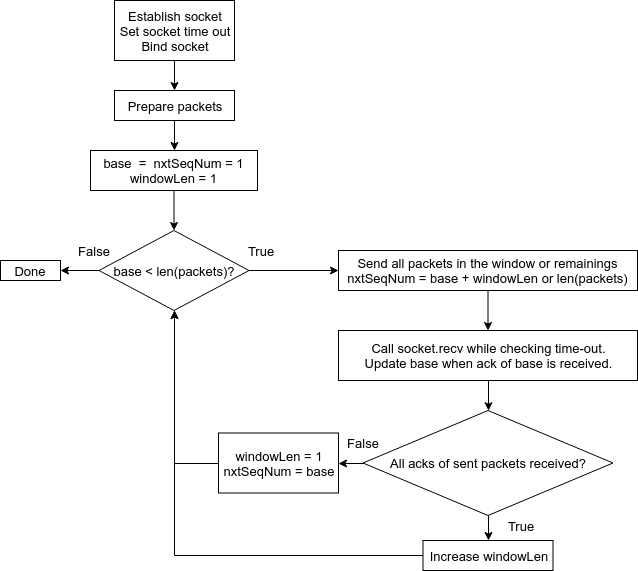
\includegraphics[width=0.55\textwidth]{Sender.png}
 \caption{Flow of Sender.}
\end{figure}

\begin{figure}[h]
 \centering
 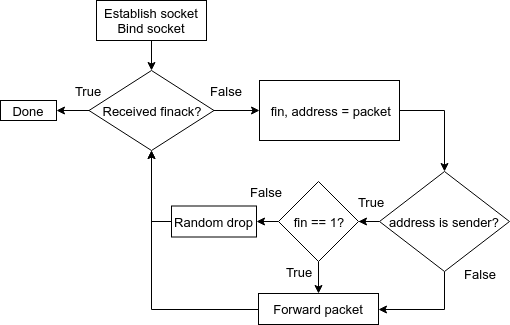
\includegraphics[width=0.47\textwidth]{Agent.png}
 \caption{Flow of Agent.}
\end{figure}

\begin{figure}[h]
 \centering
 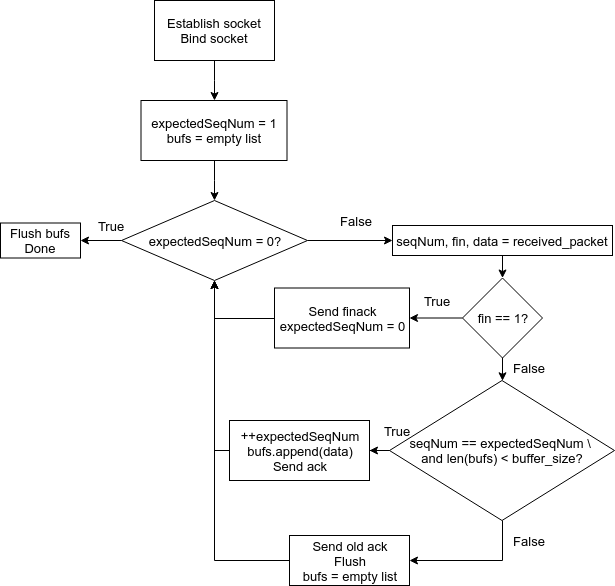
\includegraphics[width=0.52\textwidth]{Receiver.png}
 \caption{Flow of Receiver.}
\end{figure}

\newpage
\section{Difficulties and Solutions}
\subsection{Communication between Python and C (i.e. TA's agent.c)}
Integer in Python is not fix-sized.
Saving a Python integer naively, such as using pickle, will result in variable-sized data.
However, 32-bit integer is needed in the \texttt{header} struct in ``agent.c.''
After searching for a solution, I came across \texttt{to\_bytes} and \texttt{from\_bytes} functions that are meant to encode Python integer into fix-sized data.
Finally, after some trials and errors, I found that specifying \texttt{4}, \texttt{little-Endian} and \texttt{signed=True} in the functions' arguments solves the issue.

\subsection{Loss rate and buffer size}
After finishing ``Sender.py'' and ``Receiver.py'', I realize that my \texttt{winSize} never reaches 3.
At first, I thought there may be some bugs.
However, after reviewing my code, I cannot found any major bug.
Eventually, I found that the default value of loss rate is too high, and the default value of buffer size is too low.
After setting new default values, the problem is solved.

\end{document}
